% Options for packages loaded elsewhere
\PassOptionsToPackage{unicode}{hyperref}
\PassOptionsToPackage{hyphens}{url}
\documentclass[
]{book}
\usepackage{xcolor}
\usepackage{amsmath,amssymb}
\setcounter{secnumdepth}{5}
\usepackage{iftex}
\ifPDFTeX
  \usepackage[T1]{fontenc}
  \usepackage[utf8]{inputenc}
  \usepackage{textcomp} % provide euro and other symbols
\else % if luatex or xetex
  \usepackage{unicode-math} % this also loads fontspec
  \defaultfontfeatures{Scale=MatchLowercase}
  \defaultfontfeatures[\rmfamily]{Ligatures=TeX,Scale=1}
\fi
\usepackage{lmodern}
\ifPDFTeX\else
  % xetex/luatex font selection
\fi
% Use upquote if available, for straight quotes in verbatim environments
\IfFileExists{upquote.sty}{\usepackage{upquote}}{}
\IfFileExists{microtype.sty}{% use microtype if available
  \usepackage[]{microtype}
  \UseMicrotypeSet[protrusion]{basicmath} % disable protrusion for tt fonts
}{}
\makeatletter
\@ifundefined{KOMAClassName}{% if non-KOMA class
  \IfFileExists{parskip.sty}{%
    \usepackage{parskip}
  }{% else
    \setlength{\parindent}{0pt}
    \setlength{\parskip}{6pt plus 2pt minus 1pt}}
}{% if KOMA class
  \KOMAoptions{parskip=half}}
\makeatother
\usepackage{longtable,booktabs,array}
\usepackage{calc} % for calculating minipage widths
% Correct order of tables after \paragraph or \subparagraph
\usepackage{etoolbox}
\makeatletter
\patchcmd\longtable{\par}{\if@noskipsec\mbox{}\fi\par}{}{}
\makeatother
% Allow footnotes in longtable head/foot
\IfFileExists{footnotehyper.sty}{\usepackage{footnotehyper}}{\usepackage{footnote}}
\makesavenoteenv{longtable}
\usepackage{graphicx}
\makeatletter
\newsavebox\pandoc@box
\newcommand*\pandocbounded[1]{% scales image to fit in text height/width
  \sbox\pandoc@box{#1}%
  \Gscale@div\@tempa{\textheight}{\dimexpr\ht\pandoc@box+\dp\pandoc@box\relax}%
  \Gscale@div\@tempb{\linewidth}{\wd\pandoc@box}%
  \ifdim\@tempb\p@<\@tempa\p@\let\@tempa\@tempb\fi% select the smaller of both
  \ifdim\@tempa\p@<\p@\scalebox{\@tempa}{\usebox\pandoc@box}%
  \else\usebox{\pandoc@box}%
  \fi%
}
% Set default figure placement to htbp
\def\fps@figure{htbp}
\makeatother
\setlength{\emergencystretch}{3em} % prevent overfull lines
\providecommand{\tightlist}{%
  \setlength{\itemsep}{0pt}\setlength{\parskip}{0pt}}
\usepackage[]{natbib}
\bibliographystyle{apalike}
\usepackage{booktabs}
\usepackage{amsthm}
\makeatletter
\def\thm@space@setup{%
  \thm@preskip=8pt plus 2pt minus 4pt
  \thm@postskip=\thm@preskip
}
\makeatother
\usepackage{bookmark}
\IfFileExists{xurl.sty}{\usepackage{xurl}}{} % add URL line breaks if available
\urlstyle{same}
\hypersetup{
  pdftitle={Manual de usuario de MonitorEO-UGR},
  pdfauthor={Observatorio de Cambio Global de Sierra Nevada (Universidad de Granada)},
  hidelinks,
  pdfcreator={LaTeX via pandoc}}

\title{Manual de usuario de MonitorEO-UGR}
\author{Observatorio de Cambio Global de Sierra Nevada (Universidad de Granada)}
\date{2025-02-19}

\begin{document}
\maketitle

{
\setcounter{tocdepth}{1}
\tableofcontents
}
\chapter{Introduccion}\label{introduccion}

MonitorEO-UGR es una herramienta de análisis de variables derivadas de teledetección satelital basada en Google Earth Engine desarrollada por el Observatorio de Cambio Global de Sierra Nevada (Universidad de Granada).

\chapter{Interfaz grafica}\label{interfaz-grafica}

\pandocbounded{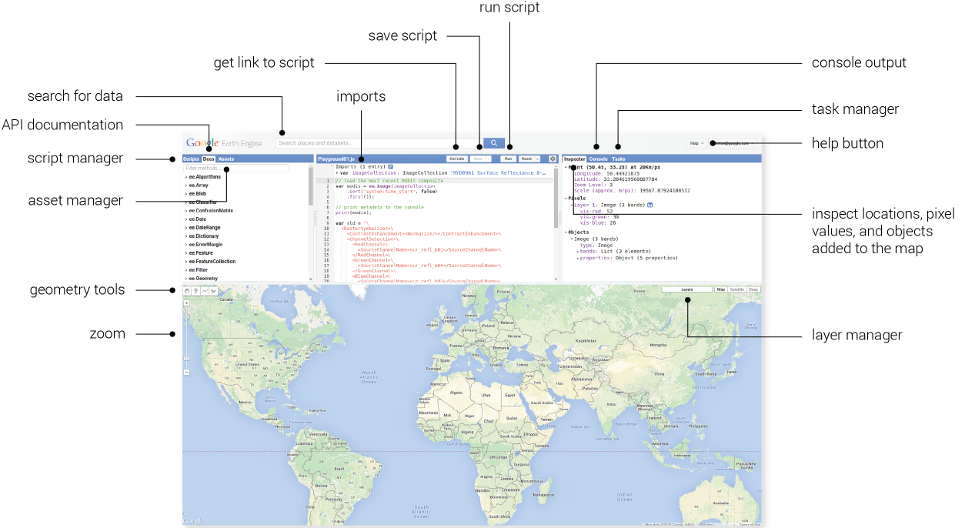
\includegraphics[keepaspectratio]{assets/annotated_playground.png}}

\chapter{Idiomas}\label{idiomas}

xxx

\chapter{Area de estudio}\label{area-de-estudio}

xxx

\chapter{Fechas de inicio y fin}\label{fechas-de-inicio-y-fin}

xxx

\chapter{Seleccion de un intervalo especifico}\label{seleccion-de-un-intervalo-especifico}

xxx

\chapter{Tipo de variable de interes}\label{tipo-de-variable-de-interes}

xxx

\chapter{Variable especifica}\label{variable-especifica}

xxx

\chapter{Sensor satelital}\label{sensor-satelital}

xxx

\chapter{Unidad temporal de agregacion}\label{unidad-temporal-de-agregacion}

xxx

\chapter{Metricas de agregacion espacial}\label{metricas-de-agregacion-espacial}

xxx

\chapter{Filtrado de nubes}\label{filtrado-de-nubes}

xxx

\chapter{Generar mapas y graficos de resultados}\label{generar-mapas-y-graficos-de-resultados}

\bibliography{book.bib,packages.bib}

\end{document}
